\subsection{Nivel de abstracción 1: Módulos principales}

  \paragraph{}El nivel de abstracción 1 muestra una visión general de los
  módulos principales de los que se compone la aplicación: Administrador
  principal, Administrador de centro, Asesores y Alumnos.

  \begin{description}
   \item[Módulo de Administrador principal]
   \item[Módulo de Administrador de centro]
   \item[Módulo de Asesores]
   \item[Módulo de Alumnos]
  \end{description}

  \paragraph{}La figura \ref{diagramaNivel1} muestra el nivel de abstracción 1.

        \begin{figure}[!ht]
            \begin{center}
            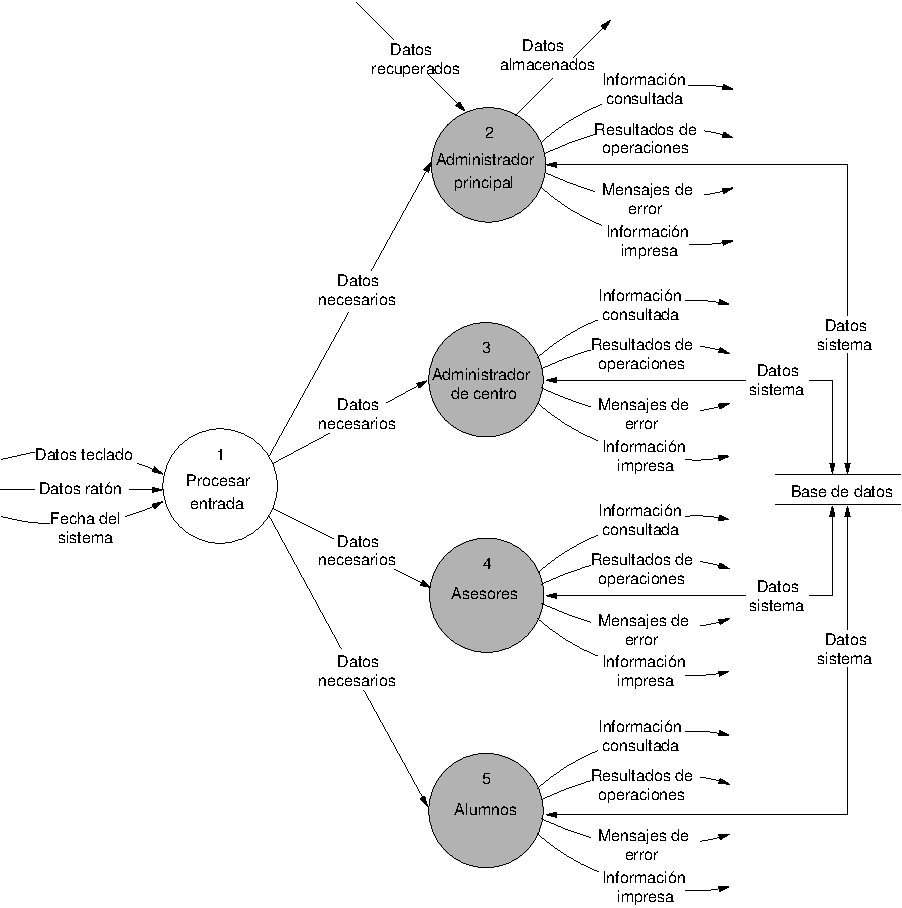
\includegraphics[]{08.Analisis_Funcional/8.2.DFDs/Niveles/Diagramas/nivel1.pdf}
            \caption{Nivel de abstracción 1: Módulos principales.}
            \label{diagramaNivel1}
            \end{center}
         \end{figure}